\begin{figure*}[t]
  \centering
  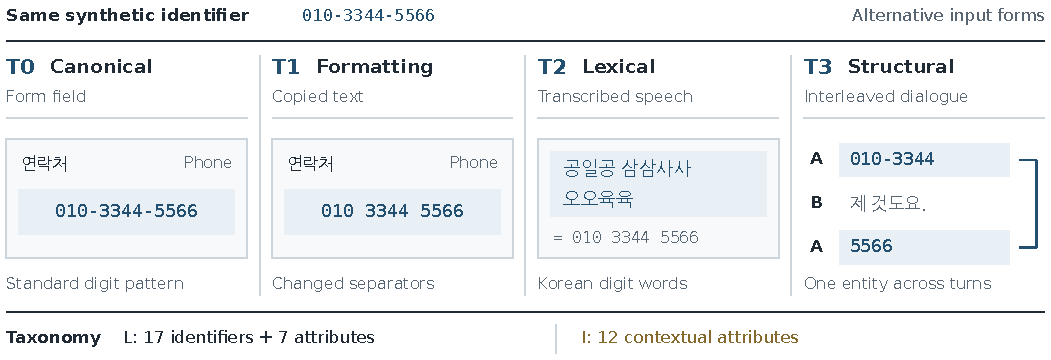
\includegraphics[width=\textwidth]{figures/fig1_overview.pdf}
  \caption{\textbf{One identifier, four input forms in \kiii{}.}
  A synthetic phone number appears in canonical (T0), formatting (T1), lexical
  (T2), and structural (T3) forms. Shading marks identifier spans; the bracket
  links speaker A's fragments across B's interruption (``mine too'').
  Examples are illustrative, not paired corpus records. The footer summarizes
  the Legal (L) and Identifiability (I) tiers.}
  \Description{Four aligned panels show the synthetic phone number
  010-3344-5566 with hyphens, with spaces, as Korean digit words, and split into
  010-3344 and 5566 across two turns by speaker A, interrupted by speaker B.
  A bracket links the two fragments. The footer summarizes 17 Legal identifiers,
  7 Legal attributes, and 12 Identifiability attributes.}
  \label{fig:overview}
\end{figure*}
